\documentclass{article}
\usepackage{graphicx} % Required for inserting images
\usepackage[top=0.9in, bottom=1in, left=1.5in, right=1.5in]{geometry}
\usepackage[utf8]{inputenc}
\usepackage[icelandic]{babel}
\usepackage[T1]{fontenc}
\usepackage[sc]{mathpazo}
\usepackage[parfill]{parskip}
\renewcommand{\baselinestretch}{1.2}
% Tables and lists
\usepackage{booktabs,tabularx}
\usepackage{multirow}
\usepackage{enumerate}
\usepackage{adjustbox}
\usepackage{multicol}
\usepackage{xcolor}
\usepackage{algpseudocode}
\usepackage{tikz}
\usepackage{nicefrac}
\usepackage{changepage}
\usetikzlibrary{arrows, positioning, calc, graphs}

% Math
\usepackage{amsmath, amsfonts, amssymb, amsthm}
% Graphics

\usepackage{graphicx}
\usepackage{tikz}
% Code environment
\usepackage{minted}
%\usepackage{bm}
%\usepackage{siunitx}
%\usepackage{animate}
\usepackage{hyperref}
%\usepackage{movie15}
%\usepackage{multicol}
%\usepackage{changepage}
\title{Tölvugrafík Verkefni 2}
\author{Ragnar Björn Ingvarsson, rbi3}
\tikzset{->, >=stealth', shorten >=1pt, node distance=2cm,thick, main node/.style={circle,draw,minimum size=3em}}

\begin{document}
\renewcommand\thepage{}
	
	\maketitle

	\newpage
	\setcounter{page}{1}
	\renewcommand\thepage{\arabic{page}}

	\part{Verkefnislýsing}

	Í þessu verkefni á að skrifa WebGL forrit til að sýna og herma 
	Lífsleikinn (Game of life) eftir John Conway í \textbf{þrívídd}, á 
	10x10x10 grind. Þar sem leikurinn er í þrívídd eru 26 nágrannar hvers 
	kubbs í stað þeirra 8 í tvívídd. Þess vegna notum við þær reglur að 
	hvert tómt hólf helst tómt nema séu nákvæmlega 6 nágrannar og hvert 
	lifandi hólf helst lifandi ef nágrannar eru 5, 6 eða 7, annars deyr það. 
	Hvert hólf á að vera teningur og dauð hólf eru bara tóm. Notandinn á 
	svo að geta snúið grindinni í hringi og hreyft sig inn og út. 
	Engin grind á að sjást en hver teningur á að vera aðeins minni en 
	hólfin í grindinni, 
	svo einstakir teningar sjáist greinilega. Einnig þarf að láta teningana 
	minnka og stækka smátt og smátt þegar þeir birtast eða hverfa. Til að 
	byrja með skal velja lifandi teninga af handahófi með um $20\%$ líkum.

	\part{Mín útfærsla}

	Til að halda utan um grindina nota ég þrívíðu fylkin \textit{cubes} og 
	\textit{prevCubes} fyrir hvernig grindin er núna og hvernig hún var í 
	síðustu ítrun. Til að byrja með fylli ég \textit{cubes} af núllum fyrir 
	dauða reiti og ásum fyrir lifandi reiti, með $20\%$ líkum á að vera 
	lifandi, og fylli \textit{prevCubes} með núllum. 

	Síðan nota ég sama kóða og notaður var fyrir verkefnin í fyrra heimadæmi 
	til að fá kubb litaðan á mismunandi hátt á hverri hlið og byrja svo 
	ítranirnar og teikna.

	Ítranirnar virka svo að ég nota \textit{setTimeout} á tveggja sekúndna 
	millibili og kalla aftur á fallið eftir að tíminn er liðinn. Í hverri 
	ítrun þá afrita ég \textit{cubes} inn í \textit{prevCubes} með for 
	lykkju og síðan, með annarri for lykkju fer ég í gegn um hvern kubb í 
	\textit{prevCubes} og tel nágranna hans. Síðan athuga ég hvort kubburinn 
	sé lifandi og nágrannar séu 5, 6 eða 7 eða þá hvort kubburinn sé dáinn 
	og nágrannar séu 6. Ef annaðhvort gengur þá bitwise XOR-a ég viðeigandi 
	\textit{cubes} kubb við $1$ til að skipta um stöðu. Eftir þetta eru 
	komnar tvær grindur, gamla og nýja. Einnig endurræsi ég \textit{tween} 
	gildið í $0$ í hverri ítrun sem verður mikilvægt til að teikna.

	Til að telja nágranna nota ég for lykkju í gegn um 3x3x3 grind kring um 
	hvern kubb. Síðan, fyrir hvern kubb taldan tek ég modulus af hnitunum 
	plús $10$ til að gera ráð fyrir hólfum út við enda og láta þau telja 
	nágranna á hinni hliðinni.

	Loks er þá komið að því að teikna. Hér renn ég í gegn um hvert hólf
	í grindinni og athuga hvort kubbur hafi breyst frá síðustu ítrun til 
	núna. Ef svo er ekki teikna ég hann bara eins og alltaf. Hins vegar ef 
	svo er, þá nota ég gildin \textit{s\_in} og \textit{s\_out} frá 
	föllunum \textit{bounce\_curve} og \textit{exp\_curve}. Þessi föll eru 
	notuð til að fá mismunandi easing curves fyrir kubba að birtast og 
	kubba að hverfa. Ég nota \textit{tween} gildið til að reikna hversu 
	langt hreyfingin er komin og bæti þá $0.1$ við það í hvert skipti sem 
	ég teikna og stoppa það svo þegar það kemst í $1$. Svo kasta ég þessum 
	gildum í skölunarfylki til að reikna hversu stór kubburinn verður. Þetta 
	lætur kubbana birtast og hverfa á betri hátt en að bara blikka inn og út 
	og er líka betra en bara línuleg hreyfing.

	Þar með er allt forritið komið og svo náði ég bara í kóða frá fyrrum 
	verkefnum til að bæta við skrunun inn og út og eiginleikanum að getað 
	snúið grindinni um með músinni.

	\vspace{2em}
	\begin{center}
		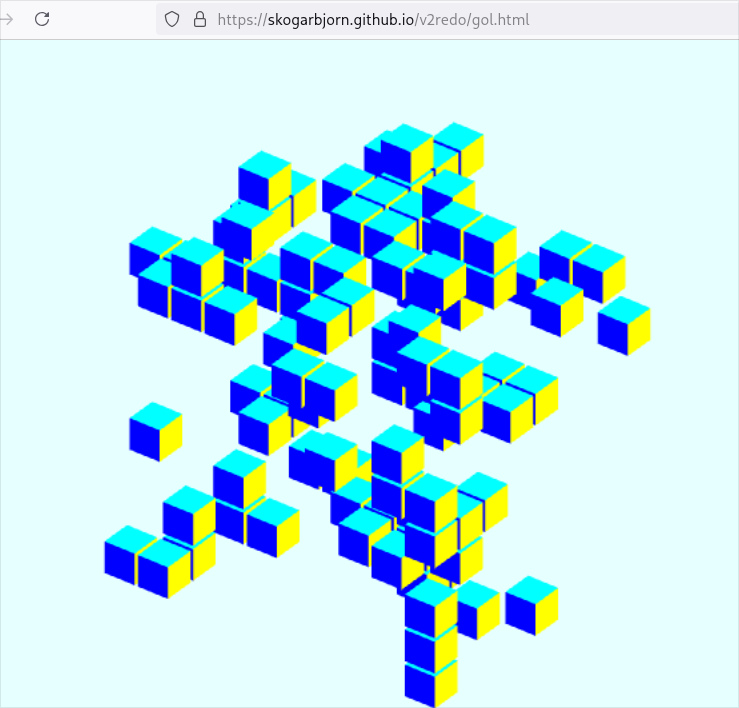
\includegraphics[scale=0.45]{demo.png}

		\url{https://skogarbjorn.github.io/v2redo/gol.html}
	\end{center}
\end{document}
